
This chapter presents the results of our experiments, including a description of the dataset, evaluation metrics, parameter settings, and a detailed analysis of the results. The discussion includes the social and cultural impact of the work, error analysis, and limitations of the dataset.

\section{Dataset Description}

The success of deep learning systems in real-world applications heavily depends on access to high-quality, diverse, and well-annotated datasets. In our work on cassava disease classification, we have used a publicly available dataset originally released as part of a Kaggle competition focused on cassava leaf disease detection.

The dataset contains a total of 21,367 labeled images with an original resolution of $512 \times 512 \times 3$, which we resized to $224 \times 224 \times 3$ to match the input requirements of standard deep learning models. The images primarily consist of cassava leaves collected in real-world farming environments by local farmers. Each sample was later annotated by experts from the National Crops Resources Research Institute (NaCRRI) in collaboration with Makerere University's Artificial Intelligence Lab.

This classification task involves five output categories: four common cassava diseases and one representing healthy leaves. Each image is associated with one of the following class labels:

\begin{itemize}
    \item \textbf{0: Cassava Bacterial Blight (CBB)} – 867 images. Shows symptoms such as blight, wilting, dieback, and vascular necrosis. Infected leaves exhibit angular necrotic markings, sometimes surrounded by chlorotic rings.
    \item \textbf{1: Cassava Brown Streak Disease (CBSD)} – 1,716 images. Caused by CBSV and UCBSV viruses, and leads to chlorosis and necrotic patterns on leaves. This disease is most prevalent in East Africa.
    \item \textbf{2: Cassava Green Mottle (CGM)} – 1,868 images. First reported in the Solomon Islands, CGM causes puckering and discoloration (yellow spots, green mosaics) in young leaves. Though plants may recover, growth is often stunted.
    \item \textbf{3: Cassava Mosaic Disease (CMD)} – 10,403 images. Characterized by distorted leaves and chlorotic (mosaic-like) patches. It is caused by single-stranded DNA viruses such as ACMV, EACMV, and SACMV, spread by whiteflies.
    \item \textbf{4: Healthy} – 2,044 images. Leaves appear uniformly dark green with no visible disease symptoms.
\end{itemize}

\vspace{0.4cm}
\noindent\textbf{Class Distribution Summary:}

\begin{table}[H]
\centering
\begin{tabular}{|l|c|}
\hline
\textbf{Class Name} & \textbf{Number of Images} \\
\hline
Cassava Mosaic Disease (CMD) & 10,403 \\
Cassava Green Mottle (CGM)   & 1,868 \\
Cassava Brown Streak Disease (CBSD) & 1,716 \\
Cassava Bacterial Blight (CBB) & 867 \\
Healthy & 2,044 \\
\hline
\textbf{Total} & \textbf{21,367} \\
\hline
\end{tabular}
\caption{Distribution of samples in each cassava disease class.}
\label{tab:class_distribution}
\end{table}

Figures~\ref{fig:cbb} to~\ref{fig:cmd} present visual examples of the five dataset categories, offering a comprehensive illustration of all cassava leaf conditions included in the dataset.

\begin{figure}[H]
    \centering
    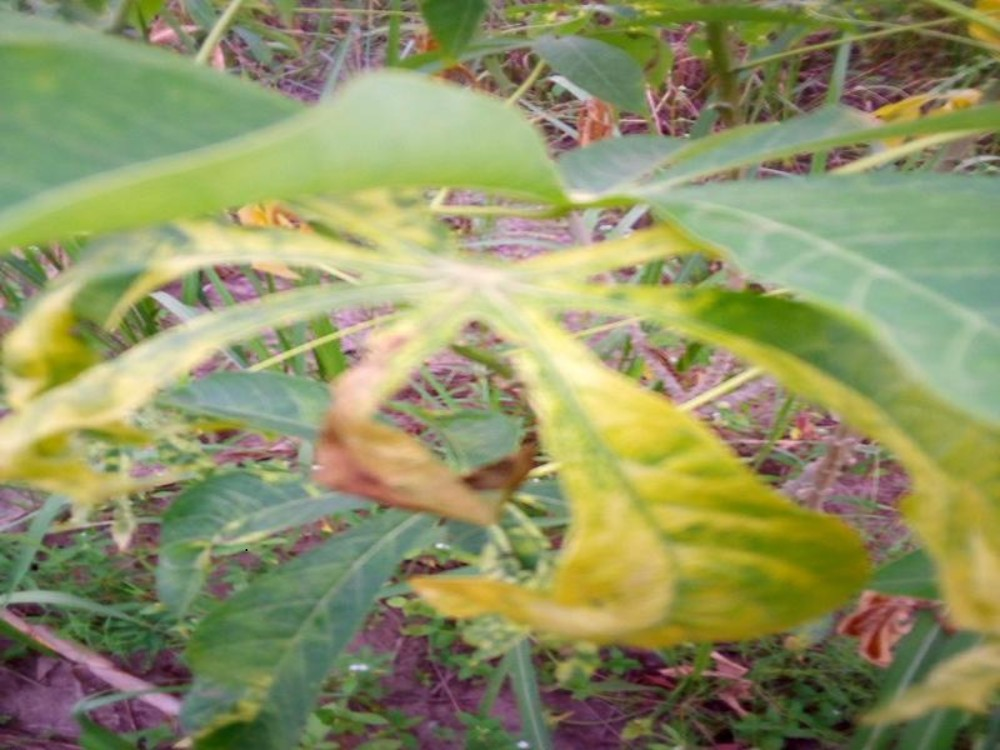
\includegraphics[width=0.7\linewidth]{figures/cbb.jpg}
    \caption{Cassava Bacterial Blight (CBB)}
    \label{fig:cbb}
\end{figure}

\begin{figure}[H]
    \centering
    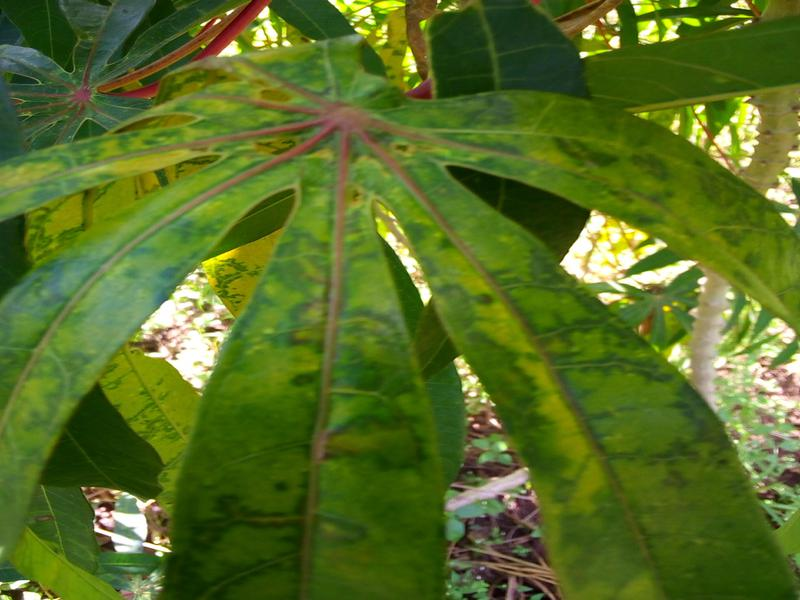
\includegraphics[width=0.7\linewidth]{figures/cbsd.jpg}
    \caption{Cassava Brown Streak Disease (CBSD)}
    \label{fig:cbsd}
\end{figure}

\begin{figure}[H]
    \centering
    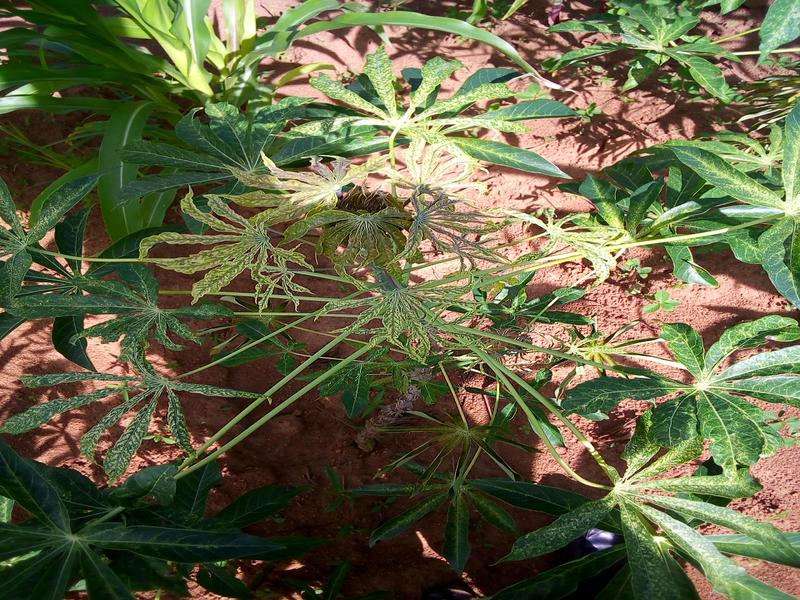
\includegraphics[width=0.7\linewidth]{figures/cgm.jpg}
    \caption{Cassava Green Mottle (CGM)}
    \label{fig:cgm}
\end{figure}

\begin{figure}[H]
    \centering
    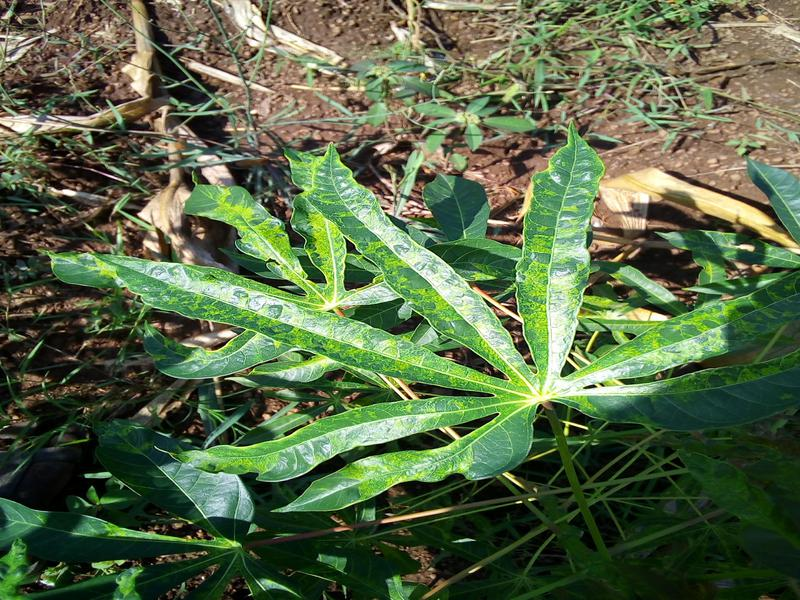
\includegraphics[width=0.7\linewidth]{figures/cmd.jpg}
    \caption{Cassava Mosaic Disease (CMD)}
    \label{fig:cmd}
\end{figure}

\begin{figure}[H]
    \centering
    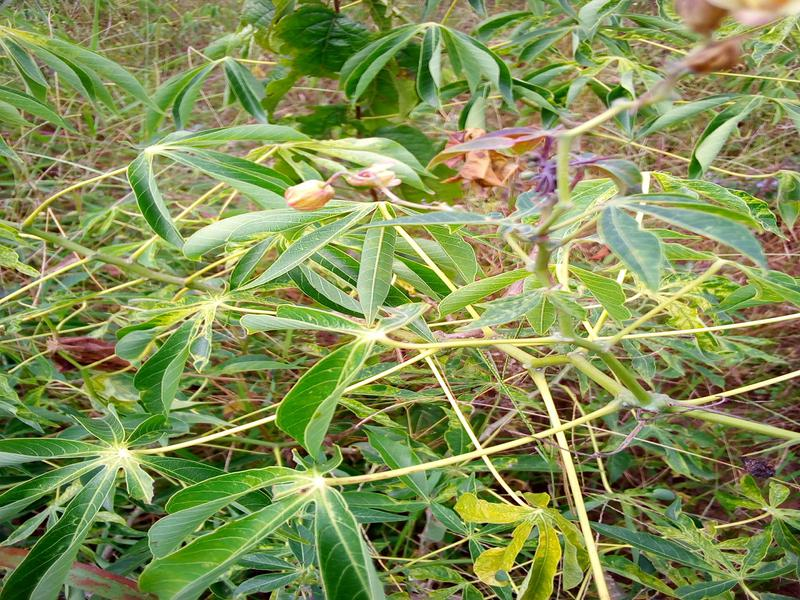
\includegraphics[width=0.7\linewidth]{figures/healthy.jpg}
    \caption{Healthy}
    \label{fig:healthy}
\end{figure}

\begin{figure}[H]
  \centering
  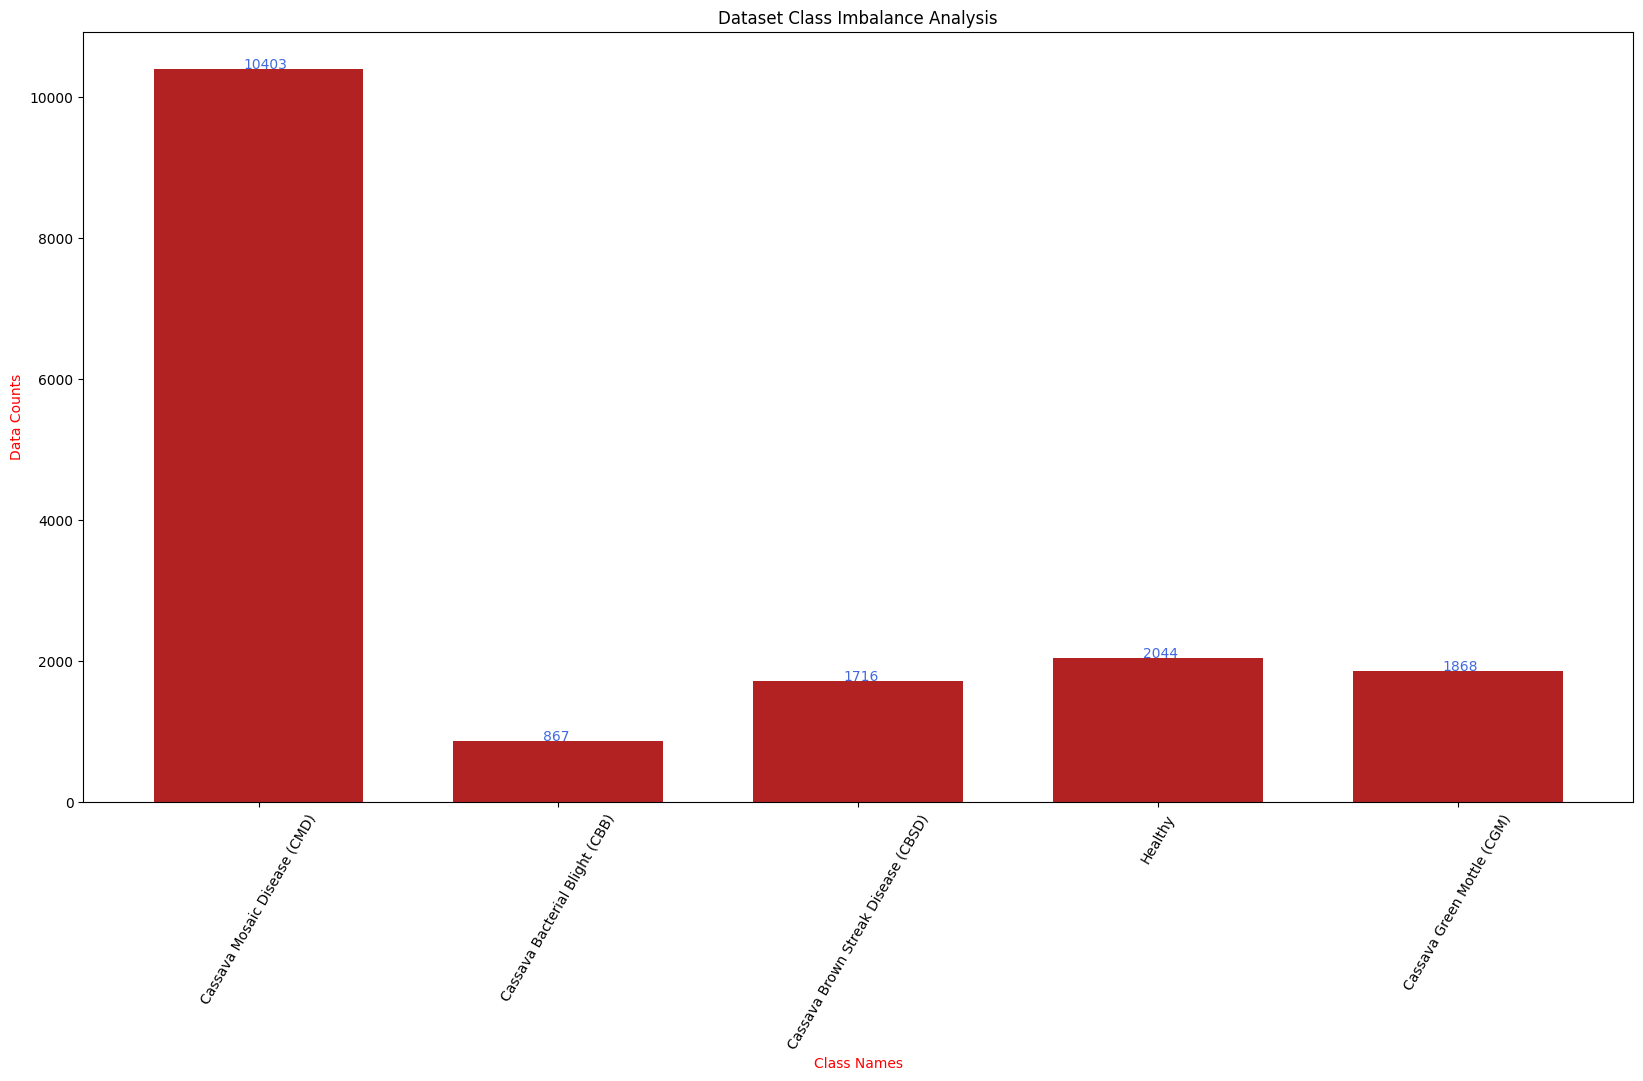
\includegraphics[width=1.0\linewidth]{figures/data_chart.png}
  \caption{Dataset Class Imbalance Analysis Chart}
  \label{fig:cmd}
\end{figure}


This dataset poses a realistic challenge for automated classification systems due to variations in lighting, leaf orientation, and background noise — all typical of on-field image collection. Thus, it serves as a strong foundation for developing robust, real-world cassava disease detection models.



This dataset poses a realistic challenge for automated classification systems due to variations in lighting, leaf orientation, and background noise — all typical of on-field image collection. Thus, it serves as a strong foundation for developing robust, real-world cassava disease detection models.

\section{Evaluation Criteria}
We used the following evaluation metrics to assess model performance:
\begin{itemize}
  \item \textbf{Accuracy:} Proportion of correctly classified images.
  \item \textbf{F1-Score:} The harmonic mean of precision and recall, which is more informative than accuracy in imbalanced datasets.
  \item \textbf{Confusion Matrix:} A matrix showing the distribution of predicted and actual class labels, providing insights into misclassifications.
\end{itemize}

\section{Parameter Settings}
For all models, we used the following hyperparameters:
\begin{itemize}
  \item \textbf{Optimizer:} Adam optimizer with default parameters ($\beta_1=0.9$, $\beta_2=0.999$).
  \item \textbf{Learning Rate:} Starting at $1 \times 10^{-3}$, reduced on plateau by a factor of 0.5.
  \item \textbf{Batch Size:} 32.
  \item \textbf{Epochs:} 8 epochs, with early stopping if validation loss did not improve for 5 epochs.
  \item \textbf{Loss Function:} Categorical Cross-Entropy.
  \item \textbf{Regularization:} Dropout layer with a rate of 0.5 in the classifier head.
\end{itemize}

\section{Experimental Results}
Table~\ref{tab:results} summarizes the validation accuracy and F1-Score for each model. As shown, **ReXNet150** outperformed all other models, achieving the highest validation accuracy and F1-Score.

\begin{table}[H]
  \centering
  \begin{tabular}{lcc}
    \toprule
    \textbf{Model}       & \textbf{Val.\ Accuracy (\%)} & \textbf{Val.\ F1–Score (\%)} \\
    \midrule
    Xception             & 91.3                         & 91.0                          \\
    EfficientNetB0       & 91.1                         & 90.8                          \\
    ResNet50             & 85.0                         & 84.6                          \\
    VGG16                & 68.0                         & 67.5                          \\
    DenseNet121          & 87.0                         & 86.8                          \\
    InceptionV3          & 86.4                         & 86.0                          \\
    \textbf{ReXNet150}   & \textbf{94.7}                & \textbf{94.9}                 \\
    \bottomrule
  \end{tabular}
  \caption{Validation accuracy and F1-Score for all models.}
  \label{tab:results}
\end{table}

\begin{figure}[H]
  \centering
  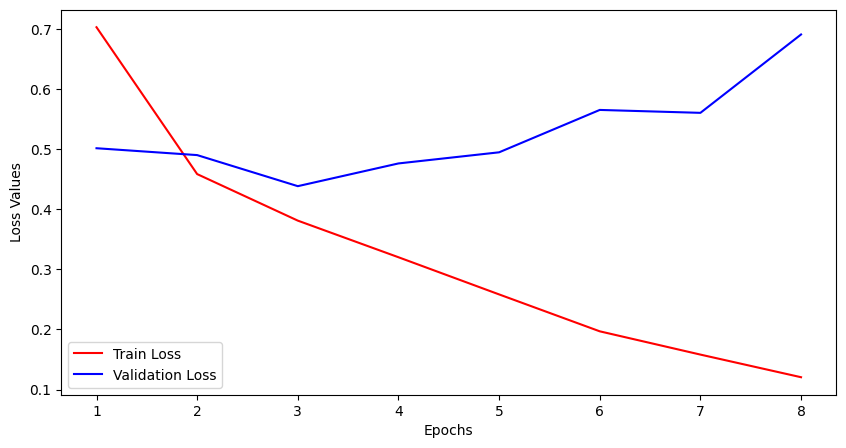
\includegraphics[width=0.8\textwidth]{figures/ac1.png}
  \caption{Training vs. Validation Accuracy across epochs for ReXNet150.}
  \label{fig:acc_curve}
\end{figure}

\begin{figure}[H]
  \centering
  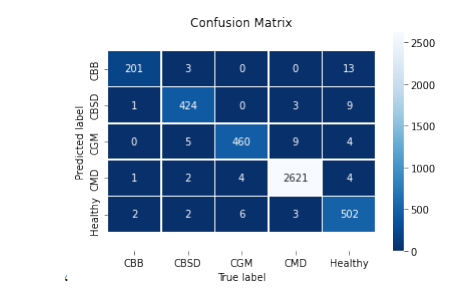
\includegraphics[width=0.9\textwidth]{figures/mtx.png}
  \caption{Confusion matrix for ReXNet150 on the validation set.}
  \label{fig:conf_matrix}
\end{figure}

\section{Discussion}
\subsection{Social and Cultural Impact}
Cassava is a crucial crop for millions of smallholder farmers, particularly in regions like sub-Saharan Africa and Southeast Asia, where it serves as a staple food. The proposed automated cassava leaf disease classification system has several significant impacts:
\begin{itemize}
  \item \textbf{Improved Food Security:} Early detection of diseases like CBB and CBSD can help farmers implement timely interventions, reducing crop loss and ensuring a stable food supply.
  \item \textbf{Empowerment of Farmers:} A mobile-based diagnostic tool based on this model can empower farmers by providing them with easy-to-use, cost-effective, and timely disease identification solutions, especially in remote areas where access to experts is limited.
  \item \textbf{Sustainable Agriculture:} Targeted disease management reduces the need for excessive pesticide use, which can help preserve the environment and reduce the overall cost of farming.
\end{itemize}

\subsection{Error Analysis and Limitations}
While the model shows high performance, there are several areas where errors could arise and limitations in the dataset:
\begin{itemize}
  \item \textbf{Class Imbalance:} Although the dataset is balanced in terms of the number of samples per class, real-world data may exhibit class imbalance, especially in less common diseases. The model may struggle to identify these underrepresented classes accurately.
  \item \textbf{Similar Visual Features:} Diseases like Cassava Green Mottle (CGM) and CBB share similar visual symptoms, which can lead to misclassifications, particularly when the disease manifests in less obvious forms. This issue is reflected in the confusion matrix (Figure~\ref{fig:conf_matrix}).
  \item \textbf{Field Image Variability:} The dataset includes images captured in varying field conditions, with differences in lighting, resolution, and background noise. These factors may reduce model accuracy when deployed in real-world environments, where image quality can vary significantly.
  \item \textbf{Generalization to New Environments:} The model was trained on a specific set of cassava leaf images, and its performance may decrease when applied to new datasets or different geographical locations due to variations in leaf morphology and disease progression.
\end{itemize}

In future work, we aim to address these limitations by:
\begin{itemize}
  \item Augmenting the dataset with more diverse images from different regions.
  \item Using semi-supervised learning techniques to leverage unlabeled data and improve generalization.
\end{itemize}